\chapter[Referencial Teórico]{Referencial Teórico}

\section{Transição demográfica}
Segundo \citeonline{omran_epidemiologic_2005}, a transição demográfica é um conceito que descreve as mudanças ocorridas nos padrões demográficos de uma população ao longo do tempo. Essas mudanças estão associadas à transição de uma estrutura populacional caracterizada por altas taxas de mortalidade e natalidade para uma estrutura em que tanto a mortalidade quanto a natalidade são baixas.

% A transição demográfica normalmente ocorre em quatro fases distintas. Conforme mencionado por \citeonline{vasconcelos_transicao_2012}, a primeira fase é caracterizada por uma sociedade pré-industrial, onde as taxas de natalidade e mortalidade são altas e praticamente se equilibram. A segunda fase marca o início da transição, com uma queda nas taxas de mortalidade, mas a natalidade permanece alta. A terceira fase é a transição propriamente dita, onde a taxa de natalidade começa a diminuir devido a fatores como urbanização, educação e acesso a métodos contraceptivos. No entanto, como a mortalidade continua a cair, a população continua a crescer, embora em um ritmo mais lento do que na segunda fase. Finalmente, a quarta fase é caracterizada por baixas taxas de natalidade e mortalidade, resultando em um crescimento populacional estável ou mesmo em declínio.

O esquema geral do crescimento populacional decorrente da evolução da natalidade e da mortalidade foi originalmente descrito em 1847 pela função logística de Verhust e em 1909 por Landry \cite{patarra1986}. Posteriormente, em 1934, Landry revisou esse trabalho, identificando os três períodos do processo: primitivo, intermediário e contemporâneo. Em 1945, Notestein introduziu o conceito de Transição Demográfica, descrevendo suas fases: pré-transição, transição e pós-transição. \citeonline{landry1982} e \citeonline{notestein1945} desenvolveram o conceito clássico da transição demográfica, que se refere à mudança das altas para as baixas taxas de mortalidade e fecundidade, resultando em diferentes fases no processo.


De acordo com \citeonline{patarra1986}, \citeonline{silva2010} e \citeonline{oliveira2015} a ideia inicial da primeira transição demográfica, que começou nos finais do século XVIII, baseia-se principalmente na experiência europeia e é caracterizada pela transição de uma sociedade tradicional e rural para uma sociedade moderna e urbano-industrial, impulsionada por transformações sanitárias, alimentares, médicas, tecnológicas e socioeconômicas.

O conceito da Segunda Transição Demográfica, apresentado por Van de Kaa e Lesthaeghe em 1986, descreve uma nova fase da história demográfica, especialmente observada em países da Europa Ocidental e industrializados a partir dos anos 1960. A característica principal é o "controle total sobre a fecundidade", com a redução da taxa de natalidade mantida abaixo do nível de reposição geracional de 2,1 filhos por mulher segundo \citeonline{vandekaa2002}. Essa segunda transição é impulsionada por mudanças nas normas e atitudes em relação à sociedade moderna, à família e aos filhos.

Em relação à mortalidade, a primeira transição demográfica é marcada por uma queda acentuada na mortalidade infantil, enquanto na segunda transição, ocorre um aumento na expectativa de vida, mais rápido do que o esperado. Como resultado, a mortalidade muda de predominar nas idades mais jovens para as idades mais avançadas. Segundo \cite{vandekaa2002}, a imigração também se torna um fator importante no crescimento populacional durante a segunda transição.

No período pós-transicional, a redução contínua da fecundidade, o envelhecimento da população e a redefinição do modelo familiar nas sociedades industrializadas avançadas levam à necessidade de imigração para manter o equilíbrio demográfico.

Embora a aplicação de uma teoria geral para explicar os padrões demográficos em contextos diferentes tenha sido criticada, de acordo com \citeonline{peixoto2007} as regularidades observadas justificam o reconhecimento dos vários contributos teóricos para a compreensão da "transição".

A dimensão espacial dos processos demográficos foi enfatizada por \citeonline{zelinsky1971}, que destacou a importância da mobilidade na compreensão do processo de modernização. Ele argumentou que as transições demográficas e migratórias são interdependentes e ocorrem em paralelo, influenciando outros processos socioeconômicos. O autor também observou que o termo "transição demográfica" refere-se apenas às mudanças nos nascimentos e mortes, enquanto a verdadeira transição demográfica resulta da interação entre as transições vitais e migratórias.

No contexto brasileiro, observa-se uma queda acentuada na taxa de fecundidade ao longo do século XX. Uma dessas mudanças foi a diminuição da taxa de mortalidade seguida pela diminuição na taxa de fecundidade \cite{beltrao_dinamica_2004}. Na década de 1960, o país apresentava uma taxa de fecundidade de 5,8 filhos por mulher, enquanto em 2021 esse número reduziu para 1,76 filhos, de acordo com dados do IBGE \cite{noauthor_ibge_nodate}.


\begin{figure}[H]
    \centering
    \includegraphics[width=0.8\textwidth]{figuras/envelhecimento_projecao.pdf}
    \caption{Projeção de envelhecimento populacional. \\
    Fonte: \cite{noauthor_ibge_nodate}.}
    \label{fig:envelhecimento}
\end{figure}

Além disso, a redução das taxas de fecundidade e mortalidade, aliada ao aumento da expectativa de vida, contribuiu para o envelhecimento da população brasileira. Segundo \citeonline{vasconcelos_transicao_2012}, o índice de envelhecimento populacional no Brasil aumentou de 10,3\% na década de 1950 para 44,8\% em 2010, e tende a aumentar cada vez mais conforme aponta a pirâmide demográfica na projeção do IBGE, atualizada em 2018, apresentada na Figura \ref{fig:envelhecimento}.

\section{Pessoa idosa}
A definição de pessoa idosa varia de acordo com as diferenças socioeconomicas de cada país. Segundo a Organização Mundial da Saúde (OMS), classificam-se como pessoas idosas indivíduos com mais de 65 anos em países desenvolvidos e com mais de 60 anos que países em desenvolvimento.
No Brasil, o Art. 1º da Lei nº 10.741, sancionada em 1 de outubro de 2003, institui o Estatuto da Pessoa Idosa, destinado a regular os direitos assegurados a essa população \cite{lei10741}. O Art. 2º da Lei nº 8.842, sancionada em 04 de janeiro de 1994, dispõe sobre a criação da política nacional do idoso, que tem como objetivo "assegurar os direitos sociais do idoso"\cite{lei8842}. Segundo ambas leis, são definidas como idosas pessoas com idade igual ou superior a 60 anos. 

O crescimento da população idosa representa uma tendência que vêm acontecendo no Brasil no século XXI. Segundo Indicadores e Dados Básicos (IDB) divulgados pelo Departamento de Informática do Sistema Único de Saúde \cite{DATASUS2012}, essa população compreende o total de 20.889.849 indivíduos.

\section{Uso de tecnologia por pessoas idosas}

Segundo \citeonline{kachar2002terceira}, ocorreram mudanças significativas no perfil dos idosos recentemente. No passado, era mais habitual que os idosos se retirassem para seus aposentos e passassem o resto de suas vidas dedicados aos netos e rememorando suas lembranças. No entanto, nos dias atuais, os idosos demonstram maior vitalidade e aspiram a envolver-se em projetos futuros, contribuir para a produção e até mesmo participar ativamente das transformações sociais e políticas. 

Atualmente, existe cada vez mais incentivo para que as pessoas idosas se familiarizem com o uso da Internet. A utilização da web oferece benefícios significativos para a qualidade de vida e o bem-estar dos idosos, permitindo a comunicação com familiares e amigos, a realização de pesquisas e outras atividades que promovem uma maior independência. No entanto, é comum que muitos idosos tenham receio de utilizar a Internet devido a problemas e padrões desconhecidos encontrados durante sua utilização, uma vez que muitos sistemas são projetados focados apenas no público jovem, que já possui maior familiaridade com a web \cite{rodrigues2018support}.

No ano de 2021, 57,5\% das pessoas com 60 anos ou mais utilizavam a Internet no Brasil, em comparação a 44,8\% no ano de 2019, como apresenta a Figura \ref{fig:uso_Internet}.

\begin{figure}[H]
    \centering
    \includegraphics[width=0.8\textwidth]{figuras/uso_da_Internet_grupos_etarios.pdf}
    \vspace{-40pt}
    \caption{Uso da Internet no Brasil por grupos etários. \\
    Fonte: \citeonline{ibge_acesso_a_Internet}.}
    \label{fig:uso_Internet}
\end{figure}

Segundo a mesma pesquisa, 71,2\% das pessoas com 60 anos ou mais utilizavam o telefone móvel celular no Brasil no ano de 2021, em comparação a 66,6\% no ano de 2019, como apresenta a Figura \ref{fig:uso_celular}.
\vspace{-10pt}
\begin{figure}[H]
    \centering
    \includegraphics[width=0.8\textwidth]{figuras/uso_celular.pdf}
    \vspace{-40pt}
    \caption{Uso do telefone móvel celular no Brasil por grupos etários.\\ 
    Fonte: \citeonline{ibge_acesso_a_Internet}.}
    \label{fig:uso_celular}
\end{figure}

Portanto, conforme apresentado por \citeonline{ibge_acesso_a_Internet} e \citeonline{sixsmith_older_2022}, houve um aumento no uso de TICs por idosos durante o período da pandemia de COVID-19. Segundo \citeonline{sixsmith_older_2022}, esse aumento ocorre principalmente devido à necessidade de comunicação social, especialmente devido à pandemia e ao isolamento social, onde as pessoas idosas foram restritas a se comunicarem através do uso de tecnologia.

Conforme destacado por \citeonline{lima2007idoso}, é essencial que a população idosa seja encorajada a adquirir conhecimentos sobre as novas tecnologias. A Internet representa uma oportunidade de romper com a zona de conforto do idoso e direcioná-lo para novas formas de aprendizado, capazes de aprimorar sua qualidade de vida. Apesar dos benefícios oferecidos pela tecnologia, de acordo com \citeonline{kachar2002terceira}, a população idosa frequentemente enfrenta dificuldades para se adaptar à nova linguagem e acompanhar os avanços tecnológicos, inclusive em tarefas básicas como utilizar eletrodomésticos, celulares e caixas eletrônicos, o que pode levar à exclusão social dessa faixa etária. 


\section{Qualidade de Software}

A computação vem sendo aplicada em diversas áreas, sendo, dessa forma, importante desenvolver software de alta qualidade \citeonline{ISO/IEC25000}. Segundo \citeonline{159342}, Software é definido como "programas de computador, procedimentos e possivelmente documentação associada e dados relacionados à operação de um sistema de computador". Softwares podem apresentar falhas e erros, sendo assim necessário assegurar a qualidade do software. A \citeonline{159342} sugere como definição de Qualidade de Software:
\begin{quote}
O grau em que um sistema, componente ou processo atende a requisitos específicos; e \\
O grau em que um sistema, componente ou processo atende às necessidades ou expectativas do cliente ou usuário.
\end{quote}

Além dessa definição, existem diversas outras definições de qualidade de software. \citeonline{pressman2016engenharia} refere-se a qualidade de software como a aplicação de uma gestão adequada, de forma a criar um produto que forneça valor aos que o desenvolvem e aos que o utilizam, além de cumprir os requisitos esperados pelos usuários. Segundo essa definição, existem três requisitos que devem ser atendidos pelo desenvolvedor para a garantia de qualidade de software \citeonline{galin_software_2004}:

\begin{itemize}
    \item Requisitos funcionais específicos;
    \item Os bons padrões de software mencionados no contrato;
    \item Boas práticas de Engenharia de Software (GSEP), garantindo a adoção de práticas profissionais de vanguarda, que devem ser cumpridas pelo desenvolvedor, mesmo que não estejam explicitamente mencionadas no contrato.
\end{itemize}

\subsection{Normas SQuaRE}
Segundo a \citeonline{ISO/IEC25000}, a série de normas ISO/IEC 25000 forma um conjunto de normas conhecido como SQuaRE (\textit{Systems and software Quality Requirements and Evaluation}).
As normas SQuaRE têm como objetivo auxiliar desenvolvedores e compradores de software na especificação e avaliação dos requisitos de qualidade. Essa série de normas dispõe de um conjunto de métricas de qualidade que pode ser utilizado para avaliar a qualidade do produto \citeonline{ISO/IEC25000}.
\vspace{-20pt}
\begin{figure}[H]
    \centering
    \includegraphics[width=1.0\textwidth]{figuras/square_board.pdf}
    \vspace{-40pt}
    \caption{Modelo de Qualidade: Normas SQuaRE.\\
    Fonte: adaptado de \citeonline{ISO/IEC25000}.}
    \label{fig:qualidade-produto}
\end{figure}

As normas SQuaRE são divididas em:

\begin{itemize}
  \item Divisão de Gestão da Qualidade (ISO/IEC 2500n): As normas dessa divisão definem todos os modelos, termos e definições referenciados por outras normas da série SQuaRE \citeonline{ISO/IEC25000}.
  \item Divisão de Modelo de Qualidade (ISO/IEC 2501n): As normas dessa divisão apresentam um modelo de qualidade do produto, incluindo a qualidade interna, externa e de uso. Além disso, um guia prático do uso do modelo de qualidade é disponibilizado \citeonline{ISO/IEC25000}.
  \item Divisão de Medição da Qualidade (ISO/IEC 2502n): As normas dessa divisão definem um modelo de medição de qualidade de um produto de software, definições matemáticas e um guia prático para sua aplicação. Além disso, as métricas apresentadas se aplicam à qualidade de software interna, externa e de uso \citeonline{ISO/IEC25000}.
  \item Divisão de Requisitos de Qualidade (ISO/IEC 2503n): As normas dessa divisão têm como objetivo auxiliar na especificação dos requistos de qualdiade, de forma que pode ser utilizado no processo de elicitação de requisitos de qualidade de um produto de software ou como insumo de um processo de avaliação de qualidade \citeonline{ISO/IEC25000}.
  \item Divisão de Avaliação da Qualidade (ISO/IEC 2504n): As normas dessa divisão dispõem de requisitos, recomendações a \textit{guidelines} para avaliação do produto de software \citeonline{ISO/IEC25000}.
\end{itemize}

A avaliação de produtos de software, a fim de satisfazer as necessidades de qualidade do software, é um dos processos no ciclo de vida do desenvolvimento de software. Neste contexto, a qualidade do produto de software pode ser avaliada medindo a qualidade interna do software, medindo a qualidade externa do software ou medindo a qualidade do software em uso, tendo como objetivo que o produto se comporte como esperado em um contexto de utilização específico \citeonline{ISO/IEC25000}. 

Deste modo, a qualidade do processo contribui para melhorar a qualidade do produto, e a qualidade do produto contribui para melhorar a qualidade em uso. Portanto, avaliar e melhorar um processo é um meio de aprimorar a qualidade do produto, assim como avaliar e melhorar a qualidade do produto é um meio de aprimorar a qualidade em uso. Da mesma forma, avaliar a qualidade em uso pode fornecer feedback para melhorar um produto, assim como avaliar um produto pode fornecer feedback para melhorar um processo \citeonline{ISO/IEC25000}.

\begin{figure}[H]
    \centering
    \includegraphics[width=0.9\textwidth]{figuras/quality_types.pdf}
    \vspace{-40pt}
    \caption{As influências entre os tipos de qualidade (processo, produto e em uso).\\
    Fonte: Adaptado de \citeonline{ISO/IEC25000}.}
    \label{fig:relacao-qualidades}
\end{figure}

A qualidade do produto influencia diretamente na qualidade em uso, conforme retrata a Figura \ref{fig:relacao-qualidades}. Deste modo, o foco desse trabalho é abordar a qualidade do produto.

\subsection{ISO/IEC 25010}

A ISO/IEC 25010 descreve o modelo de qualidade para o produto de software interno, externo e em uso, apresentando características e subcaracterísticas de qualidade \citeonline{ISO/IEC25000}. As características de qualidade são divididas em 8: Adequação funcional, Desempenho e Eficiência, Compatibilidade, Usabilidade, Confiabilidade, Segurança, Manutenibilidade e Portabilidade \citeonline{ISO/IEC25010}.

\begin{figure}[H]
    \centering
    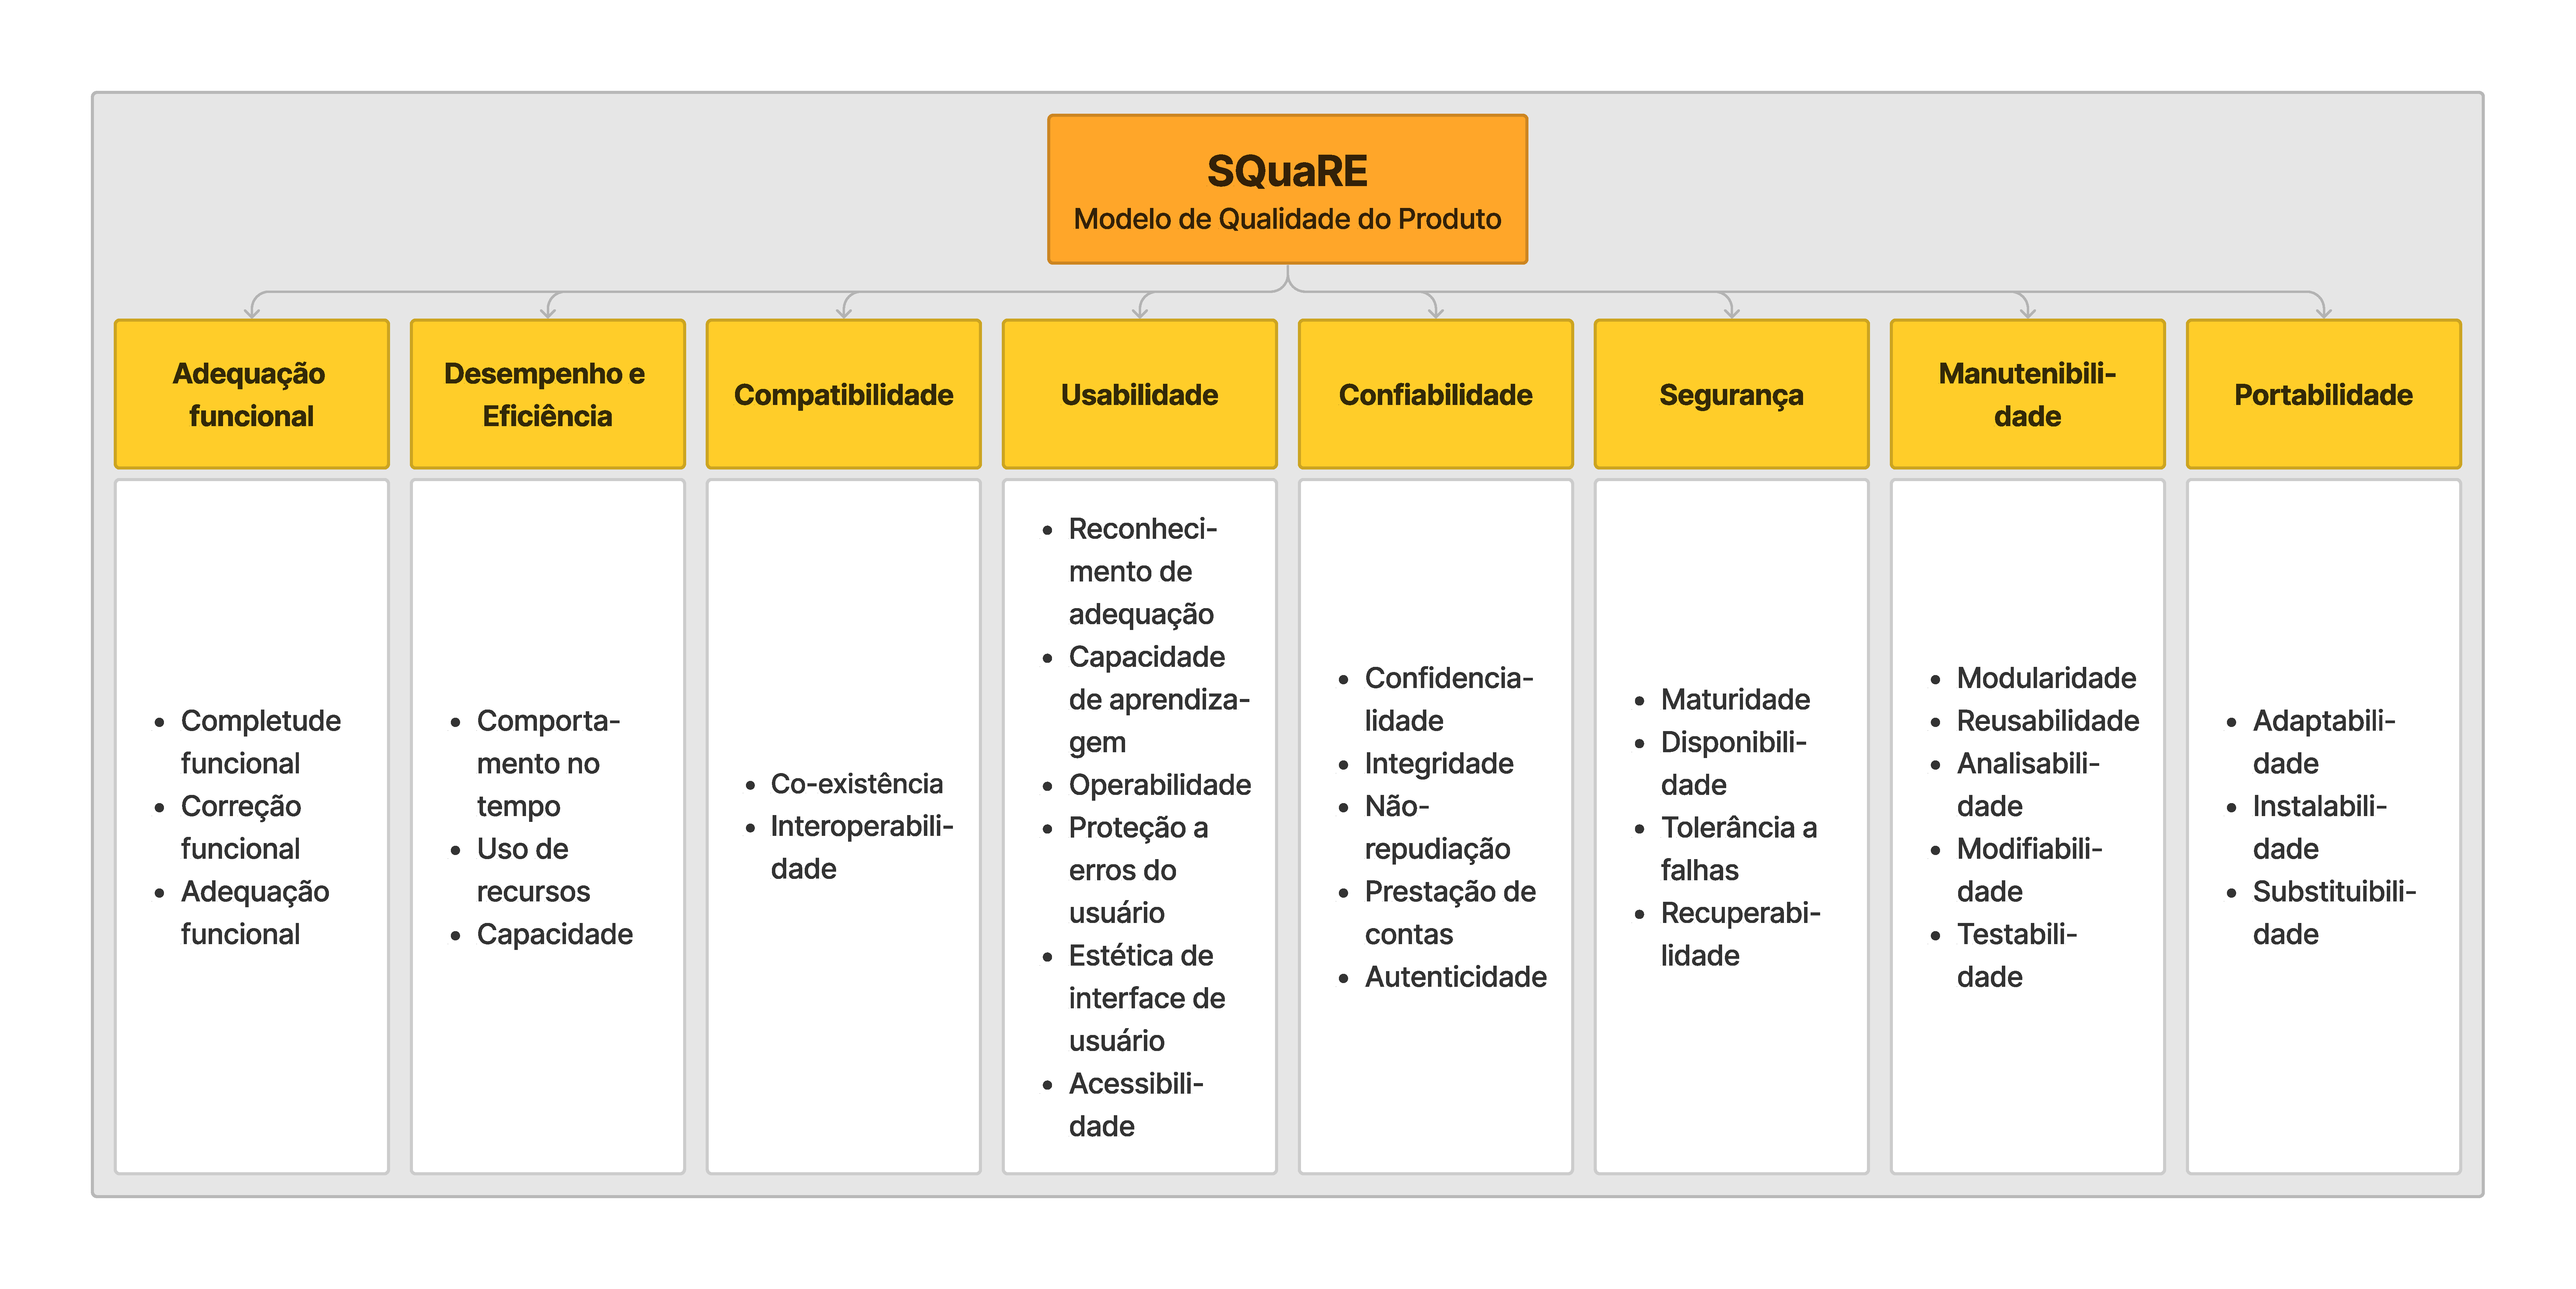
\includegraphics[width=1.0\textwidth]{figuras/Untitled.pdf}
    \vspace{-25pt}
    \caption{Qualidade do produto.\\
    Fonte: \citeonline{ISO/IEC25010}.}
    \label{fig:qualidade-produto}
\end{figure}

\subsubsection{Adequação Funcional}

Adequação Funcional é definida como a capacidade de um produto ou sistema de oferecer funções que atendem às necessidades declaradas e implícitas quando usado em condições especificadas \citeonline{ISO/IEC25010}. Essa característica de qualidade é composta das seguintes subcaracterísticas:

\begin{itemize}
  \item Completude funcional: é o grau em que um conjunto de funcionalidades atende os objetivos e tarefas do usuário \cite{ISO/IEC25010}.
  \item Correção funcional: é o grau em que um produto ou sistema dispõe de resultados corretos, dado um grau de precisão \citeonline{ISO/IEC25010}.
  \item Adequação funcional: é o grau em que as funções facilitam a realização de tarefas e objetivos especificados \citeonline{ISO/IEC25010}.
\end{itemize}

\subsubsection{Desempenho e Eficiência}

Desempenho e Eficiência é definida como o desempenho de um software em relação à quantidade de recursos utilizados sob condições estabelecidas \cite{ISO/IEC25010}. Essa característica de qualidade é composta das seguintes subcaracterísticas:

\begin{itemize}
  \item Comportamento no tempo: é o grau em que os tempos de resposta e processamento, assim como as taxas de transferência, de um produto ou sistema, ao desempenhar suas funções, atendem aos requisitos.
  \item Uso de recursos: é o grau em que as quantidades e tipos de recursos utilizados por um produto ou sistema, ao desempenhar suas funções, atendem aos requisitos.
  \item Capacidade: é o grau em que os limites máximos de um parâmetro de um produto ou sistema atendem aos requisitos estabelecidos.
\end{itemize}

\subsubsection{Compatibilidade}

Compatibilidade é definida como a capacidade de um produto, sistema ou componente poder trocar informações com outros produtos, sistemas ou componentes, e/ou desempenhar suas funções requeridas, enquanto compartilha o mesmo ambiente de hardware ou software \citeonline{ISO/IEC25010}.

\begin{itemize}
  \item Co-existência: é a capacidade de um sistema de realizar funções definidas dado que ele compartilha ambiente ou recursos com outros produtos \citeonline{ISO/IEC25010}.
  \item Interoperabilidade: é a capacidade do sistema de trocar informações e usá-las no sistema \citeonline{ISO/IEC25010}.
\end{itemize}

\subsubsection{Usabilidade}

Usabilidade é definida como a capacidade de um sistema de ser usado pelos usuários, de forma que alcancem os objetivos especificados com efetividade, eficiência e satisfação \citeonline{ISO/IEC25010}. 

\begin{itemize}
    \item Reconhecimento de adequação: é a capacidade de um sistema de ser avaliado, de forma que o usuário possa reconhecer se ele está adequado para as suas necessidades \citeonline{ISO/IEC25010}.
    \item Aprendibilidade: é a capacidade em que a utilização do sistema pode ser aprendida pelo usuário \citeonline{ISO/IEC25010}.
    \item Operabilidade: é a capacidade de um sistema de ser operado pelo usuário de forma fácil \citeonline{ISO/IEC25010}.
    \item Proteção a erros do usuário: é a capacidade de um sistema de proteger os usuários de erros \citeonline{ISO/IEC25010}.
    \item Estética de interface de usuário: é a capacidade de um sistema de dispor de uma interação de usuário agradável e satisfatória \citeonline{ISO/IEC25010}.
    \item Acessibilidade: é a capacidade de um sistema de ser usado por pessoas com a mais ampla gama de características e habilidades \citeonline{ISO/IEC25010}.
\end{itemize}

\subsubsection{Confiabilidade}

Confiabilidade é definida como a capacidade de um sistema de desempenhar funções definidas sob condições específicas \citeonline{ISO/IEC25010}.

\begin{itemize}
    \item Maturidade: é a capacidade de um sistema de satisfazer as necessidades de confiabilidade \citeonline{ISO/IEC25010}.
    \item Disponibilidade: é a capacidade de um sistema de estar acessível e ser operável sempre que necessário \citeonline{ISO/IEC25010}.
    \item Tolerância a falhas: é a capacidade de um sistema de funcionar como esperado, mesmo diante de falhas \citeonline{ISO/IEC25010}.
    \item Recuperabilidade: é a capacidade de um sistema de recuperar dados afetados e reestabelecer o estado desejado do sistema \citeonline{ISO/IEC25010}.
\end{itemize}

\subsubsection{Segurança}

Segurança é definida como a  capacidade de um sistema de proteger os dados dos usuários, garantindo que apenas pessoas ou outros sistemas com os tipos e níveis de autorização adequados tenham acesso aos dados restritos \citeonline{ISO/IEC25010}.

\begin{itemize}
    \item Confidencialidade: é a capacidade de um sistema de restringir o acesso a dados apenas para pessoas que tenham acesso autorizado \citeonline{ISO/IEC25010}.
    \item Integridade: é a capacidade de um sistema de impedir acesso não autorizado ou modificações do sistema ou de seus dados \citeonline{ISO/IEC25010}.
    \item Não-repudiação: é a capacidade de um sistema de garantir que ações ou eventos tenham sua ocorrência comprovada, de modo que não possam ser negados posteriormente \citeonline{ISO/IEC25010}.
    \item Prestação de contas: é a capacidade de um sistema de rastrear as ações de um ator, de modo que seja possível associá-las unicamente ao ator \citeonline{ISO/IEC25010}.
    \item Autenticidade: é a capacidade de um sistema de determinar se a identidade de um recurso ou sujeito é igual à reinvidicada \citeonline{ISO/IEC25010}.
\end{itemize}

\subsubsection{Manutenibilidade}

Manutenibilidade é definida como a capacidade de um sistema de ser modificado pelos mantenedores com eficiência e efetividade \citeonline{ISO/IEC25010}.

\begin{itemize}
    \item Modularidade: é a capacidade de um sistema de ser composto por componentes, de modo que a alteração de um componente impacte minimamente os outros componentes \citeonline{ISO/IEC25010}.
    \item Reusabilidade: é a capacidade de um sistema de utilizar recursos em mais de um módulo do sistema ou na construção de outros recursos \citeonline{ISO/IEC25010}.
    \item Analisabilidade: é a capacidade de um software de ser analisado com eficiência e eficácia, de modo a identificar problemas, determinar a causa de falhas ou realizar análises de impacto para mudanças planejadas \citeonline{ISO/IEC25010}.
    \item Modifiabilidade: é a capacidade de um sistema de ter seus módulos alterados efetiva e eficientemente, não introduzindo defeitos ou reduzindo a qualidade \citeonline{ISO/IEC25010}.
    \item Testabilidade: é a capacidade de um sistema de ser testado, de modo a verificar se o sistema atende os requisitos definidos \citeonline{ISO/IEC25010}.
\end{itemize}

\subsubsection
{Portabilidade}

Portabilidade é definida como a capacidade de um sistema de ser transferido de um hardware ou ambiente para outro \citeonline{ISO/IEC25010}.

\begin{itemize}
    \item Adaptabilidade: é a capacidade de um sistema de ser efetiva e eficientemente adaptado para diferentes hardwares e ambientes \citeonline{ISO/IEC25010}.
    \item Instalabilidade: é a capacidade de um sistema de ser instalado ou desinstalado num ambiente \citeonline{ISO/IEC25010}.
    \item Substituibilidade: é a capacidade de um software de ser substituido por outro software com o mesmo propósito no ambiente \citeonline{ISO/IEC25010}.
\end{itemize}

A norma \citeonline{ISO/IEC25010} apresenta diversos critérios e métricas para a avaliação da qualidade do produto, fornecendo um guia claro para avaliar as dimensões da qualidade do produto. Isso é feito com o objetivo de garantir que os produtos atendam às necessidades dos usuários idosos. Por meio dessa abordagem, os desenvolvedores são capazes de criar produtos inclusivos, permitindo que os idosos participem plenamente da sociedade digital.